\chapter{Revisão de Literatura}

Neste capítulo são descritos os trabalhos que serviram de inspiração para o projeto. 
Do mesmo modo, é feito a revisão teórica das técnicas que serão aplicadas para a resolução do problema que o projeto propõe resolver.

\section{Trabalhos Relacionados}

O Deep-RL já foi aplicado anteriormente em tarefas que envolvem robótica, entre essas aplicações podem ser referenciado os trabalhos de (\citeauthor{kober2013reinforcement}, \citeyear{kober2013reinforcement}; \citeauthor{stone2005reinforcement}, \citeyear{stone2005reinforcement}).
Mnih \citeyearpar{mnih2013playing} utilizou de rede neural convolucional para estimar uma função de valor para recompensas futuras no jogos eletrônicos do Atari, essa estratégia foi chamada de \textit{Deep Q-learning}.
A \textit{Deep Q-learning} pode ser apenas usada em uma tarefa que tenha ações discretas. Para estendê-lo para o controle contínuo, Lillicrap \citeyearpar{lillicrap2015continuous} propôs uma política de gradiente determinística profunda.
Essa tornou a base para as aplicações de Deep-RL na navegação de robôs móveis, assim como, na criação de novas técnicas como actor-crítica suave \cite{haarnoja2018soft}.

Tai \citeyearpar{tai2017virtual} criou um planejador de movimento sem mapeamento para um robô móvel pegando 10 leituras de um sensor \textit{laser} e a posição de um alvo em relação ao robô como entrada, e os comandos de direção contínuos como saída da rede, mas sendo primeiramente proposto como comandos de direção discretos \cite{tai2016towards}. Foi mostrado que, com métodos assíncronos de Deep-RL, um planejador de movimento sem mapeamento pode ser treinado e completar a tarefa de chegar a um algo determinado.

Zhu \citeyearpar{zhu2017target} propôs um outro modelo para aplicar Deep-RL para a tarefa de dirigir um robô móvel. O modelo criado toma a obervação atual de estado e a imagem do alvo como entrada e gera uma ação em um ambiente de três como saída.

Uma atividade que pode ser muito desafiante na robótica é navegar um veículo com segurança e eficiência em ambientes com muitos pedestres. Chen \citeyearpar{chen2017socially} elaborou um modelo Deep-RL que pode quantificar o que fazer e não fazer no mecanismo de navegação humana.
Este trabalho desenvolveu uma politica de navegação eficiente de tempo que respeita normas sociais comuns. Criando assim um método capaz de controlar um robô móvel que se move na velocidade de caminhada humana em um ambiente com muitos pedestres.,


\section{Aprendizado de Máquina}

O aprendizado de máquina é um ramo da inteligência artificial baseada na ideia que sistemas podem aprender através de dados, identificar padrões e fazer decisões com a intervenção mínima de humanos \cite{mitchell1990machine}. Expandindo seus estudos para algoritmos e modelos estatísticos que sistemas computacionais usam para melhorar seu desempenho em tarefas específicas.

É possível classificar o aprendizado de máquina em 3 grandes categorias:
\begin{itemize}
    \item Aprendizado supervisionado: este aprendizado consiste em um sistema que possui variáveis de entrada e variáveis de saída. As variáveis de entradas são referentes a uma variável de saída determinada e o aprendizado é chamado supervisionado, pois a variável de saída, durante o treino, já é conhecida pelo algoritmo. A função desse sistema é fazer com que o algoritmo possa maximizar as predições de saída para uma resposta correta que é conhecida previamente pela rede.
    \item Aprendizado não-supervisionado: consiste em um sistema que apenas possui variáveis de entrada sem uma saída correspondente. O objetivo desse tipo de aprendizado é modelar estruturas que possam dizer mais sobre o conjunto dos dados que estão sendo estudados.
    \item Aprendizado por reforço: neste tipo de aprendizado o agente inteligente interage com um ambiente dinâmico, para desempenhar um determinado objetivo. É fornecido, ao agente, o \textit{feedback} quanto a premiações e punições, na medida em que é explorado o espaço de solução.
\end{itemize}

\subsection{Aprendizagem profunda}

A aprendizagem profunda é uma subcategoria do aprendizado de máquinas \cite{lecun2015deep}.
Semelhante ao aprendizado de máquina, o aprendizado profundo também possui aprendizado supervisionado, não-supervisionado e de reforço.
O algoritmo de aprendizagem profunda depende de redes neurais profundas. 
Redes neurais profundas podem automaticamente achar representações compactas de baixa dimensionalidade de dados com alta dimensionalidade (e.g., imagens, texto e audio) \cite{arulkumaran2017brief}.
Essas redes neurais foram baseadas no funcionamento dos neurônios do cérebro humano. 
Ou seja, o aprendizado profundo vem dá criação de redes neurais que possuem neurônios que se comunicam entre si e conseguem passar informação. 

Uma Rede Neural Profunda (DNN) consiste de múltiplas camadas de unidades de processamento não-linear (camada escondida). Ela executa a extração e transformação de características. Na Figura \ref{fig:NN} é mostrada uma DNN que consiste que três camadas: camada de entrada, camadas escondidas e camada de saída. Na camada de entrada, os neurônios são generalizados a partir de recursos que passam por sensores que percebem o ambiente. As camadas escondidas podem incluir uma ou mais camadas. A camada de saída contem a saída desejada, por exemplo, a distribuição de todas as ações possíveis.
Cada camada sucessiva da DNN usa a saída da camada anterior como entrada.
Todos os neurônios das camadas são totalmente ativados através de conexões ponderadas.

\begin{figure}[H]
\caption{Rede Neural Simples e Profunda}
\centerline{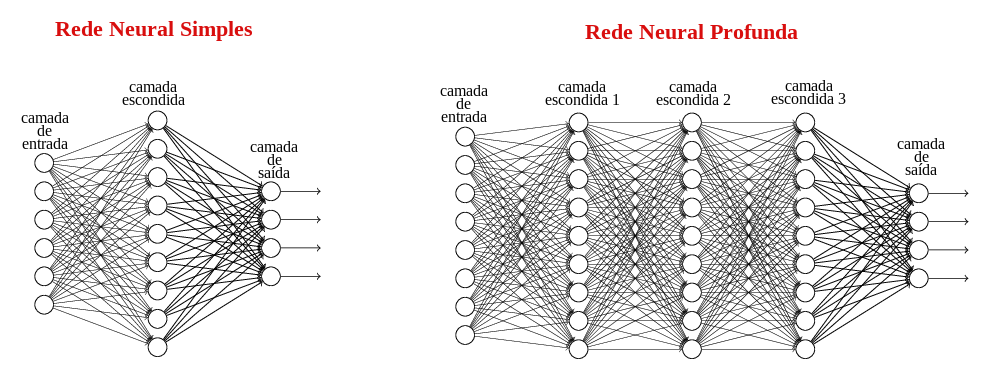
\includegraphics[width=\columnwidth]{imagens/neural_network.png}}
\small{Fonte: http://neuralnetworksanddeeplearning.com/chap5.html}
\label{fig:NN}
\end{figure}

Todas as DNN são funções matemáticas. 
Então, para calcular a função de uma camada é usado a definição abaixo:
\begin{equation}
    a^{(c)} = W a^{(c-1)} + b
    \label{eq:camada}
\end{equation}

Sendo os neurônios da camada atual $a^{(c)}$ e da camada anterior $a^{(c-1)}$, os pesos de todas as conexões entre as duas camadas $W$ e um número pré-determinado de bias $b$.

Contudo, em aplicações do mundo real, funções lineares não conseguem descrever todos os sistemas, quase sempre, funções não-lineares são usadas. Para fazer isso é preciso aplicar uma função não-linear, conhecida como função de ativação (FA), a Equação \ref{eq:camada}, que ficaria definida como:
\begin{equation}
    a^{(c)} = FA\left\{W a^{(c-1)} + b\right\}
\end{equation}

Então, para resolver sistemas não-lineares diferentes funções de ativação podem ser usadas ou pode ser criada a própria função de ativação que se ajusta ao problema. Existem diversas FA's pré-definidas, tais como: `linear', `ReLU', `tanh', `sigmoid', etc.
Na Figura \ref{fig:FA} é mostrada a respostas para as FA's mais conhecidas.

\begin{figure}[H]
\caption{Exemplos de resposta de funções de ativação}
\centerline{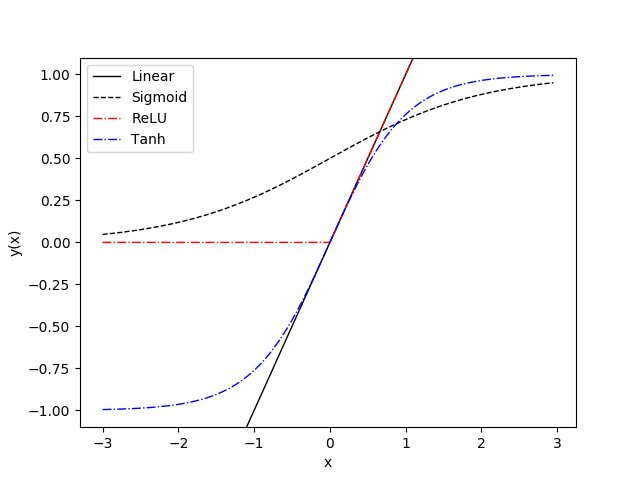
\includegraphics[width=\columnwidth]{imagens/function_activation.png}}
\small{Fonte: Autor}
\label{fig:FA}
\end{figure}

Depois do fluxo de computação avançar da entrada para a saída, na camada de saída e cada camada escondida, é possível calcular o erro derivativo para propagar os gradientes em direção a camada de entrada, sendo assim os pesos podem ser atualizados para otimizar a função de perda \cite{li2017deep}. Isto é o foco da parte de aprendizagem, para achar os pesos e bias certos.

% Geralmente utiliza-se de redes neurais e de muitos dados para o seu treinamento. 
% Essas redes neurais foram baseadas no funcionamento dos neurônios do cérebro humano. Ou seja, o aprendizado profundo vem dá criação de redes neurais que possuem neurônios que se comunicam entre si e conseguem passar informação. 
% E enquanto, programas tradicionais constroem análises com dados de uma forma linear, o aprendizado profundo constrói funções hierárquicas para o processamento de dados de uma forma não linear.

% Uma rede neural, na sua forma mais simples, é composta de múltiplas camadas de nós interconectados, como é mostrado na Figura 3. 
% As conexões da rede são similares as conexões dos neurônios do cérebro humano. 
% A conexão entre as camadas possuem um nó e a este nó está associado a um peso. 
% A rede neural é treinada pelo uso de grandes conjuntos de dados rotulados que aprendem características diretamente dos dados sem a necessidade da intervenção manual.

% figura

% A rede neural pode apresentar um maior número de camadas escondidas assim podendo-se classificar como uma rede “profunda”.
% Em uma rede neural com múltiplas camadas escondidas, o número de parâmetros cresce exponencialmente, podendo assim ter uma melhor eficiência para a resolução de problemas que uma rede neural de apenas uma única camada escondida.

% Muitos dos modelos modernos de aprendizado profundo são baseados em uma rede neural artificial. Cada nível da rede aprende a transformar as informações de entrada em algo  mais abstrato. 
% Como regra, quanto mais profunda é o modelo, mais a rede tem potencial de obter um melhor desempenho que os modelos mais superficiais. 
% O problema é que quanto mais profunda é a rede, mais dados são necessários para evitar o sobreajuste, sem falar, do aumento do tempo para obter uma resposta de saída.
% No caso de uma rede que vá cuidar de um robô, em constante movimento, é preciso ter uma resposta mais rápida. Logo, uma rede superficial é melhor para esse tipo de aplicação.

\subsection{Aprendizado por Reforço}

O aprendizado por reforço é uma área de aprendizado de máquina que lida com tomada de decisão sequencial.
Um aspecto chave do aprendizado por reforço é que um agente aprenda uma bom comportamento \cite{franccois2018introduction}.
Isso significa que ele modifica ou adquiri novos comportamentos e habilidades incrementalmente.
Um outro importante aspecto do aprendizado por reforço é que ele usa de experiência de tentativa e erro.
Ademais, o agente do aprendizado por reforço não precisa de completo conhecimento ou controle do ambiente; ele apenas precisa ser capaz de interagir com o ambiente e coletar informações.
Um agente realiza certas ações em um ambiente e um interpretador dá uma recompensa para o novo estado do agente, tendo assim um ciclo entre as ações e interpretações feitas no ambiente, como é mostrado na Figura \ref{fig:ciclo_rl}.

\begin{figure}[H]
\caption{Interação do agente no ambiente em aprendizado por reforço}
\centerline{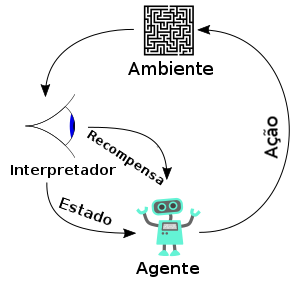
\includegraphics[width=10cm]{imagens/ciclo_rl_agente.png}}
\small{Fonte: Super Data Science}
\label{fig:ciclo_rl}
\end{figure}

O aprendizado por reforço possui dois tipos de configuração, o \textit{offline} e \textit{online} como é chamado na literatura \cite{sutton1998introduction}. Em uma configuração \textit{offline}, a experiência adquirida \textit{a priori} e então é usada para o aprendizado. Isso é um contraste com a configuração \textit{online} onde os dados tornam disponíveis em uma ordem sequencial e são usados para progressivamente atualizar o comportamento do agente.

\subsubsection{Processo de decisão de Markov}

A forma básica de modelar o aprendizado por reforço é seguindo um processo de Markov. O processo de Markov é definido como a probabilidade do estado futuro depender apenas do estado atual \cite{bellman1957markovian}. Sem depender de nenhuma das ações e estados anteriores. Isso quer dizer:
\begin{equation}
P(s_{t+1} \mid {s_0,a_0,s_1,a_1 , ... ,s_t,a_t}) = P( s_{t+1} \mid {s_t,a_t} )
\label{eq:eq1}
\end{equation}

Para um agente que está em um estado e realiza uma certa ação em um ambiente, acontecerá com que o depois dessa ação o agente se encontre em um novo estado em relação ao estado anterior, e então uma determinada recompensa é dada pela ação tomada. A função de recompensa define a meta que o agente do aprendizado por reforço deve atingir. O objetivo desse agente é maximizar a recompensa que ele recebe ao longo do tempo.

Então com a abordagem do agente que utiliza o conceito do processo de Markov, para cada tempo t, são usados os seguintes passos:
\begin{enumerate}
    \item O agente observa o estado atual $s_t$.
    \item O agente faz a ação $a_t$.
    \item O agente recebe a recompensa $r_t = R(s_t, a_t)$.
    \item O agente entra no próximo estado $s_{t+1}$.
\end{enumerate}

Sabendo que na abordagem do processo de Markov é necessário utilizar a equação de Bellman, que especifica qual é a melhor ação que um agente deve tomar em um certo estado \cite{bellman2015applied}. Isto é, a equação de Bellman consegue prever a recompensa gerada de um estado para outro, enquanto, que a função de recompensa só pensa no que é bom em um sentido imediato. A Equação de Bellman é definida como:
\begin{equation}
    V( s_{t} ) =  \underset{a_t}{max}(R(s_t,a_{t}) + \gamma V(s_{t+1}))
    \label{eq:eq2}
\end{equation}

Essa fórmula nos diz qual é o maior valor do estado depois de tomada uma ação.
`$V$' é definido como a “valor” do estado no ambiente.
O valor $\gamma$ (gama) é para admitir um valor de desconto para cada ação tomada. Com a Equação \ref{eq:eq1} e a Equação \ref{eq:eq2} definidas, considerando todas as ações possíveis que um agente pode tomar e a probabilidade de cada ação, é possível ter a equação do processo de decisão de Markov, que é definida como:
\begin{equation}
    V( s_{t} ) = \underset{a_t}{max}( R(s_t,a_{t}) + \gamma \sum_{s_{t+1}} P( s_{t+1} \mid {s_t,a_t} ) V(s_{t+1}) )
\end{equation}

Antes do processo de decisão de Markov, o que acontecia é que todas ações eram tomadas em um ambiente determinístico. Mas com a inserção de incerteza nas ações é possível modelar um ambiente de predição melhor para um lugar mais abstrato e estocástico.

\subsection{Q-Learning}

A diferença de um agente que toma suas decisões pelo processo de decisão de Markov e \textit{Q-Learning} é que em uma abordagem do Markoviana o agente olha a qualidade dos estados futuros baseados no estado atual, enquanto que em \textit{Q-Learning} o agente olha para a qualidade de cada ação sabendo o estado atual \cite{watkins1992q}. 
‘Q’ é definido como a “qualidade” da ação de um agente em um estado e a função retornada é a recompensa dessa ação. É possível derivar a fórmula para o \textit{Q-Learning} através da abordagem de Markov, gerando a seguinte equação:
\begin{equation}
    Q( s_{t}, a_t ) = R(s_t,a_{t}) + \gamma \sum_{s_{t+1}} P( s_{t+1} \mid {s_t,a_t} ) \underset{a_{t+1}}{max} (Q(s_{t+1}, a_{t+1}))
    \label{eq:eq4}
\end{equation}

Mesmo depois de achar o valor de `$Q$' causado por uma ação, é preciso lembrar que o agente precisa percorrer esse ambiente provavelmente mais de uma vez. 
Então se for mantida a ideia da equação \ref{eq:eq4}, nunca será possível que um agente inteligente possa aprender, pois essa fórmula permite apenas atualizar os valores de `$Q$' para uma certa ação que aconteceu no tempo atual, sem levar em conta se a ação foi boa ou ruim.
Para corrigir isso é preciso considerar uma diferença temporal e uma taxa de aprendizado ($\alpha$) para que assim seja possível que o algoritmo melhore seu desempenho com o tempo, mesmo que faça ações que não beneficiem o agente. 
Ou seja, é possível definir as seguintes equações:

\begin{enumerate}
    \item A equação da diferença temporal entre os valores de Q:
    \begin{gather}
        TD_t = \Delta Q( s_t,a_t )\\
        TD_t = R(s_t,a_{t}) + \gamma \sum_{s_{t+1}} P( s_{t+1} \mid {s_t,a_t} ) \underset{a_{t+1}}{max} (Q(s_{t+1}, a_{t+1}) - Q_{t-1}(s_{t}, a_{t}))
    \end{gather}
    
    \item A equação que atualizar o valor de Q para cada ação que passou por aquele estado:
    \begin{equation}
        Q_t ( s_t,a_t ) = Q_{ t-1 }( s_t,a_t )+ \alpha TD_t( s_t,a_t )
        \label{eq:q_function}
    \end{equation}
\end{enumerate}

Com a equação \ref{eq:q_function} definida é possível montar um agente inteligente que aprende por reforço e com o passar do tempo.

\subsection{Repetição de Experiência}

Na repetição de experiência o agente tem a possibilidade de usar uma memória de repetição que permite eficiência dos dados pela armazenação de experiências passadas do agente em ordem de ter a oportunidade de reprocessar os dados mais tarde.
Os dados salvos na memória se referem ao estado atual $s_t$, ação $a_t$, recompensa $r_t$ e próximo estado $s_{t+1}$ do agente.
Além do mais, as memórias de repetição também asseguram que as atualizações sejam feitas de dados razoavelmente estáveis guardados na memória o que na convergência da rede.

Enquanto a memória de repetição permite processar as transições de dados em diferentes ordens do que se foram experienciadas, há também a possibilidade de usar a repetição priorizada \cite{schaul2015prioritized}. Isso permite considerar transições de dados com diferentes frequências do que foram experienciadas dependendo de sua importância. Isso quer dizer, qual experiência é armazenada e qual é repetida.
A desvantagem desse método de repetição priorizada é a introdução de bias.

\subsection{Política de Gradiente}

Uma política define como um agente seleciona ações. Políticas podem ser categorizadas sobre o critério de ser tanto estacionária ou não-estacionária.
Uma política não estacionária depende no tempo de intervalo e é útil para contextos finitos onde a recompensa acumulativa que o agente procura otimizar são limitadas para um número finito de intervalos de tempo.

Políticas também podem ser categorizadas sobre um segundo critério de ser determinística ou estocástica:

\begin{itemize}
    \item No caso de ser determinística, a política é descrita por $\mu (s)$.
    \item No caso de ser estocástica, a política é descrita por $\pi (s,a)$, onde está denota a probabilidade que ação $a_t$ possa ser escolhida no estado $s_t$.
\end{itemize}

\subsubsection{Aprendizado de política-\textit{on} e política-\textit{off}}

Métodos de política-\textit{on} tentam avaliar ou melhorar a política que e usada para fazer as decisões, enquanto que o método de política-\textit{off} avalia e melhora a política diferente daquela usada para gerar dados. Em métodos baseados na política-\textit{off}, o aprendizado é bem direto quando se usa de trajetórias que necessariamente não foram obtidas sobre a política atual, mas de um diferente política de comportamento.
Nestes casos, a repetição de experiência permite o uso de experiências passadas para o aprendizado sem a introdução de bias. Ao contrário, métodos baseados na política-\textit{on} geralmente introduzem bias quando fazem uso de memórias de repetição pois as trajetórias não são obtidas somente para política atual.


% This approach is particularly well-suited
% in the case of off-policy learning as using experience from past (i.e.
% different) policies does not introduce any bias (usually it is even good
% for exploration)


\subsection{Ator-Crítica}

A política pode ser representada por redes neurais que atualizam por gradiente tanto de forma determinística ou estocástica. Para ambas formas, a política de gradiente necessita uma estimativa da função de valor da política atual. 
Uma abordagem comum é usar uma arquitetura ator-crítica, mostrada na Figura \ref{fig:actor_critic}, que consiste de duas partes: um ator e uma crítica \cite{konda2000actor}.
O ator se refere a política e a crítica para estimar a função de valor, podendo ela ser $Q(s,a)$ ou $V(s)$.
In Deep-RL, ambos o ator e a crítica podem  ser representados por aproximadores de função de rede neural não-linear.
Em resumo, pode ser dito que o a rede ator é responsável pela exploração de ações do agente no ambiente. Enquanto que para a rede da crítica é o que guia a rede ator dizendo se aquela ação é boa ou ruim. 

\begin{figure}[H]
\caption{Arquitetura Ator-Crítica}
\centerline{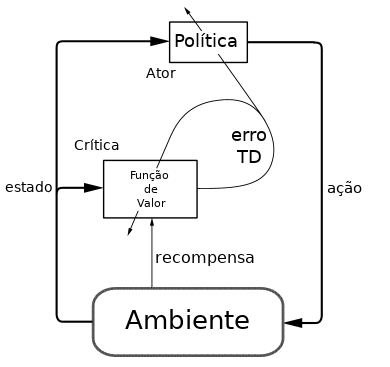
\includegraphics[width=10cm]{imagens/actor-critic_portuguese.png}}
\small{Fonte: Autor}
\label{fig:actor_critic}
\end{figure}

\subsection{Aprendizado por Reforço Profundo}

O objetivo do Aprendizado por Reforço Profundo (Deep-RL) é controlar um agente na tentativa de maximizar sua função de recompensa.
O algoritmo \textit{Deep Q-Network} \cite{mnih2013playing} foi capaz de desempenhar em nível humano muito dos jogos eletrônicos do Atari por fazer a estimativa das ações de um agente.
Contudo, enquanto a DQN pode resolver problemas em espaços de observações complexos, ela pode apenas lidar com espaços de ações discretos.
E é notável que muitas tarefas, no controle da robótica, têm espaços de ações contínuos.
Então DQN não podem ser aplicadas em domínios contínuos e é necessário usar outros algoritmos capazes de lidar com esse tipo de problema.

\subsubsection{Política de Gradiente Determinística Profunda}

O algoritmo de política de gradiente determinística profunda (DDPG) consiste de um método ator-críticab de política-\textit{off} que usa funções de aproximação que pode aprender políticas de espaço de ação contínuo.
O algoritmo faz uso de uma rede neural para a rede ator e outro para a rede crítica.
Essas duas redes computam a predição de ação para o estado atual e geram um sinal de erro de diferença temporal para cada intervalo de tempo.
A entrada da rede ator é o estado atual, e a saía é um valor real que representa uma ação escolhida para um espaço contínuo de ação.
A saída da crítica é simplesmente o valor de Q estimado do estado atual e ação dada pelo ator.

O maior desafio do aprendizado em espaço de ações contínuas é a exploração. 
Para enfrentar esse desafio é preciso construir a política de exploração $\mu'$ pela adição da amostra de ruído de um processo de ruído $\mathcal{N}$ para a política da rede ator, que é definida como:
\begin{equation}
    \mu' = \mu(s_t) + \mathcal{N}
\end{equation}

Onde $\mathcal{N}$ pode ser escolhido de um jeito que se adéqua ao ambiente. Sendo o processo de Ornstein-Uhlenbeck \cite{uhlenbeck1930theory} o mais usado para gerar eficiência de exploração correlacionada temporalmente em problemas de controle físico.

Em geral, treinar e avaliar a função de política que sai da rede ator e a função de valor que sai da rede crítica, com milhares de trajetórias simuladas correlacionadas temporalmente, leva a introdução de enormes quantidades de variância na aproximação da função verdadeira Q (crítica).
É sugerido usar uma memória de repetição para armazenar as experiências do agente durante o treino \cite{schaul2015prioritized}. 
Isto é, salvar os estados, ações, recompensas e novos estados que o agente explorou durante o episódio.
E então, aleatoriamente selecionar as experiências que vão ser usadas no aprendizado, para assim, quebrar a correlação temporal com os diferentes episódios dos treinos.

A experiência de repetição permite ao agente inteligente aprender de memórias recentes, fazendo com que aumente a velocidade de aprendizado e a quebra de correlações temporais indesejadas. Mesmo com a aplicação de uma memória curta é possível ver uma melhora substancial na desempenho do agente. 
Apesar da aplicação de uma memória de repetição deixar mais lento o aprendizado do agente, se consegue um melhor desempenho dele.

Sem contar a utilização da memória de repetição é preciso fazer uma rede alvo para gerar alvos para que o erro da diferença temporal possa ser regularizado no aprendizado do algoritmo e aumentar a estabilidade. 
A rede alvo é uma rede que possui uma cópia da rede ator e da rede crítica, porém, a sua atualização é feita de um modo “leve”.
Isso quer dizer que a rede alvo não copia diretamente os pesos da rede ator e da rede crítica. 
Os pesos, representado por $\theta$, da rede alvo são atualizados deste modo:
\begin{equation}
    \theta' \leftarrow \tau \theta + (1+\tau)\theta'
\end{equation}

Com $\tau \ll 1$ . Onde o alvo é representado pela apóstrofe.
Então o valores do alvo da rede mudam de forma lenta e assim permitem uma melhora da estabilidade do treinamento.

O algoritmo DDPG é descrito no Algoritmo \ref{alg:ddpg}. Nesta definição é possível ver com mais clareza o algoritmo de aprendizado por reforço profundo. Demonstrando toda etapa de treinamento da rede ator e da rede crítica.

% \begin{algorithm}
% \caption{DDPG com repetição de memória}
% \label{alg:ddpg}
% \begin{algorithmic}
% \STATE Aleatoriamente inicializa a rede crítica $Q(s,a|\theta^Q)$ e a rede ator $\mu(s|\theta^{\mu})$ com os pesos da rede $\theta^Q$ e $\theta^\mu$
% \STATE Inicializa a rede alvo $Q'$  e $\mu'$ com pesos $\theta^{Q'} \leftarrow \theta^Q$, $\theta^{\mu'} \leftarrow \theta^{\mu}$
% \STATE Inicializa a memória de repetição $R$
% \FOR{episódio = 1 até M}
% \STATE Inicializa um processo aleatório $\mathcal{N}$ para a ação de exploração
% \STATE Recebe o estado de observação $s_1$
% \FOR{t = 1 até T}
% \STATE Seleciona a ação $a_t = \mu(s_t|\theta^{\mu})+\mathcal{N}_t$ de acordo com a política atual e ruído de\\ exploração
% \STATE Executa a ação $a_t$ e observa a recompensa $r_t$ e observa o novo estado $s_{t+1}$
% \STATE Armazena a transição $(s_i,a_i,r_i,s_{i+1})$ em $R$
% \STATE Retira um \textit{minibatch} de amostras aleatórias de $N$ transições $(s_t,a_t,r_t,s_{t+1})$ de $R$
% \STATE Define $y_i = r_i + \gamma Q'(s_{i+1}, \mu'(s_{i+1}|\theta^{\mu'})|\theta^{Q'})$
% \ENDFOR
% \ENDFOR
% \end{algorithmic}
% \end{algorithm}

\vspace{1.5cm}
\begin{algorithm}[H]
\DontPrintSemicolon
Aleatoriamente inicializa a rede crítica $Q(s,a|\theta^Q)$ e a rede ator $\mu(s|\theta^{\mu})$ com os pesos da rede $\theta^Q$ e $\theta^\mu$. \;
Inicializa a rede alvo $Q'$  e $\mu'$ com pesos $\theta^{Q'} \leftarrow \theta^Q$, $\theta^{\mu'} \leftarrow \theta^{\mu}$. \;
Inicializa a memória de repetição $\mathcal{R}$.\;
\Para{episódio = 1 até M}{
Inicializa um processo aleatório $\mathcal{N}$ para a ação de exploração. \;
Recebe o estado de observação $s_1$.\;
\Para{t = 1 até T}{
Seleciona a ação $a_t = \mu(s_t|\theta^{\mu})+\mathcal{N}_t$ de acordo com a política atual e ruído de exploração.\;
Executa a ação $a_t$ e observa a recompensa $r_t$ e observa o novo estado $s_{t+1}$.\;
Armazena a transição $(s_t,a_t,r_t,s_{t+1})$ em $\mathcal{R}$.\;
Retira um \textit{minibatch} de amostras aleatórias de $N$ transições $(s_i,a_i,r_i,s_{i+1})$ de $\mathcal{R}$.\;
Define $y_i = r_i + \gamma Q'(s_{i+1}, \mu'(s_{i+1}|\theta^{\mu'})|\theta^{Q'})$. \;
Atualiza a rede crítica minimizando a perda: $L = \frac{1}{N} \sum_{i} (y_i - Q(s_i,a_i | \theta^Q ))^2$.\;
Atualiza a política da rede ator usando o gradiente de política da amostra retirada:\;
\begin{equation*}
    \nabla_{\theta^\mu}J  \approx  \frac{1}{N} \sum_{i} \nabla_a Q( s,a | \theta^Q ) |_{ s=s_i, a=\mu(s_i) } \nabla_{\theta^\mu}\mu( s | \theta^\mu ) |_{s_i}
\end{equation*}
Atualiza a rede alvo:
\begin{gather*}
    \theta^{ Q' } \leftarrow  \tau\theta^Q + ( 1+\tau )\theta^{ Q' }\\
    \theta^{ \mu' } \leftarrow  \tau\theta^\mu + ( 1+\tau )\theta^{ \mu' }
\end{gather*}
}
}
\caption{DDPG com repetição de memória}
\label{alg:ddpg}
\end{algorithm}
\vspace{1.0cm}

% Para melhor que representar o algoritmo, na Figura 4, foi feito um fluxograma de forma a representar o treino da rede DDPG.
% Quando o treino começa as redes crítica, ator e alvo são inicializadas de forma aleatória. 
% O treino dura no total M episódios, onde cada episódio tem T intervalos.

% \begin{figure}[H]
% \caption{Flosefes}
% \centerline{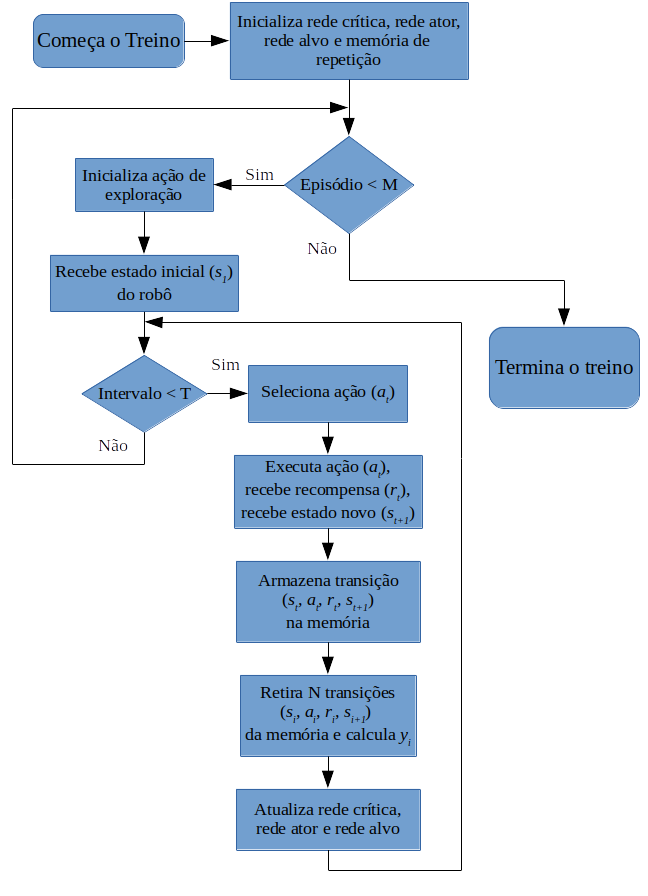
\includegraphics[width=10cm]{imagens/flowchart_ddpg.png}}
% \small{Fonte: Autor}
% \label{fig:flowchart_ddpg}
% \end{figure}

\subsubsection{Ator-Crítica Suave (SAC)}

O Ator-Crítica Suave (SAC) é um algoritmo que otimiza uma política estocástica de um modo de política-\textit{off}. A rede consiste de um método ator-crítica que usa funções de aproximação que podem aprender políticas de ação em espaços contínuos \cite{haarnoja2018soft}.
O algoritmo faz uso de uma rede neural para a rede ator, a rede valor de $V$, e outra para rede crítica.
Essas 3 redes computam a predição de ação para o estado atual e gera um sinal de erro de diferença temporal para cada intervalo de tempo.

A característica central do SAC é a regularização de entropia.
Ao invés de apenas procurar a maximização da recompensa do sistema, a SAC procura também maximizar a entropia da política.
O aumento da entropia resulta é um agente que pode explorar melhor seu ambiente, o que ajuda no aprendizado. E pode prevenir também com que uma política convirja muito cedo para um política local ótima.

A entropia se refere ao quão imprevisível uma variável aleatória pode ser.
Então, se uma variável sempre toma um único valor isso quer dizer que a entropia é considerada zero pois não é nenhum pouco imprevisível.
Uma entropia alta na política explicitamente encoraja a exploração do agente pois é atribuído uma probabilidade igual para a ação que tem o mesmo ou igual valor de $Q$ e assegura que não seja colapsado em repetidamente selecionar uma ação particular do agente.

Para calcular a entropia de $\mathcal{H}$ de uma variável aleatória $x$ de função de densidade $P$, é possível através de:
\begin{equation}
    \mathcal{H}(P) = \mathbb{E}_{x \sim P} [-\log P(x)]
\end{equation}

A rede SAC utiliza dos mesmos métodos de repetição de memória e de uma rede alvo que a rede DDPG. No Algoritmo \ref{alg:sac} é mostrado as etapas de treinamento da rede ator, da rede crítica e da rede de valor $V$ no SAC.

\vspace{1.5cm}
\begin{algorithm}[H]
\DontPrintSemicolon
Aleatoriamente inicializa a rede crítica $Q(s,a|\theta^{Q_{1}})$, $Q(s,a|\theta^{Q_{2}})$, a rede ator $\pi(s,a|\theta^{\pi})$ e a rede de valor de $V(s|\theta^V)$ com os pesos da rede $\theta^{Q_1}$, $\theta^{Q_2}$, $\theta^\pi$ e $\theta^V$. \;

Inicializa a rede alvo $V'$com pesos $\theta^{V'} \leftarrow \theta^V$\;
Inicializa a memória de repetição $\mathcal{R}$.\;

\Para{episódio = 1 até M}{
Recebe o estado de observação $s_1$.\;

\Para{t = 1 até T}{
Seleciona a ação $a_t \sim \pi(s_t,a_t|\theta^{\pi})$ de acordo com a política atual.\;

Executa a ação $a_t$ e observa a recompensa $r_t$ e observa o novo estado $s_{t+1}$.\;

Armazena a transição $(s_t,a_t,r_t,s_{t+1})$ em $\mathcal{R}$.\;

Retira um \textit{minibatch} de amostras aleatórias de $N$ transições $(s_i,a_i,r_i,s_{i+1})$ de $\mathcal{R}$.\;

Computa os alvos para a rede ator $Q$ e  $V$:
\begin{gather*}
    y_q(r_i, s_{i+1}) =  r_i + \gamma V(s_{i+1}|\theta^{V'})
    \\
    y_v (s_i) = \min_{k=1,2} Q(s_i, a_i|\theta^{Q_k}) - \alpha \log \pi (s_i, a_i|\theta^{\pi})
\end{gather*}

Atualiza a rede crítica usando o gradiente
\begin{equation*}
    \nabla_{\theta^Q_k} \frac{1}{|B|} \sum_{(s_i,a_i,r_i,s_{i+1}) \in B} (Q(s_i, a_i|\theta^{Q}_k) - y_q(r_i, s_{i+1}))^2 \qquad \textrm{for}\: k = 1,2 
\end{equation*}

Atualiza a rede valor de $V$ usando o gradiente
\begin{equation*}
    \nabla_{\theta^V} \frac{1}{|B|} \sum_{s_i \in B} (V(s_i|\theta^V) - y_v(s_i))^2
\end{equation*}

Atualiza a política da rede ator usando o gradiente
\begin{equation*}
    \nabla_{\theta^\pi} \frac{1}{|B|} \sum_{s_i \in B} (Q(s_i, a_i|\theta^{\pi}) - \alpha \log \pi (s_i, a_i|\theta^{\pi}))
\end{equation*}

Atualiza a rede valor de $V$ alvo com
\begin{gather*}
    \theta^{ V' } \leftarrow  \tau\theta^V + ( 1+\tau )\theta^{ V' }
\end{gather*}
}
}
\caption{SAC com repetição de memória}
\label{alg:sac}
\end{algorithm}
\vspace{1.0cm}

\section{Visão Computacional}

A visão computacional é ciência da computação e sistemas de \textit{software} que podem reconhecer e entender uma imagem ou cena \cite{forsyth2002computer}.
A visão computacional também é composta de vários aspectos tais como reconhecimento de imagem, detecção de objetos geração de imagem, super-resolução de imagem e mais.
Do ponto de vista da engenharia, ela procura automatizar tarefas que o sistema visual humano pode fazer.
A detecção de objetos é provavelmente o mais profundo aspecto da visão computacional devido ao grande número de casos práticos.

\subsection{Rastreamento de Objetos}

Para fazer o rastreamento de objetos primeiramente é preciso detectar um objeto.
A detecção de objetos se refere a capacidade de computadores e sistemas de \textit{software} de localizar em um imagem ou cena e de identificar cada objeto.
Sendo amplamente utilizado para detecção de faces, detecção de veículos, pedestres e carros autônomos.
Existem muitas maneiras que a detecção de objetos pode ser usada. Em muitos casos a cor do objeto é usado para sua detecção.

O rastreamento de objetos é o processo de localizar um objeto alvo movendo em quadros consecutivos de um vídeo \cite{bascle1995region}. Essa associação pode ser especialmente difícil quando o objeto se move rápido em relação a taxa de quadros do vídeo. Outra situação que aumenta a complexidade do problema é quando o objeto rastreado se move em relação ao tempo. Para essas situações geralmente são aplicados modelos de movimento em que é descrito como a imagem do alvo pode mudar para diferente movimentos dos objetos. Essas aplicações se encontram muito relacionadas com a robótica. Já que muitas aplicações usam de visão para poder completar suas tarefas.